\subsection{Risk Managment}
For this project, the ”Project Management Triangle” is lacking the cost dimension, while the time dimension is fixed (strict deadlines). As a result, any risks that appear, automatically lead to a reduction of the project scope if there is no spare time. Because of this, we will prioritize dealing with risks above regular tasks and prioritize essential tasks over nice-to-haves, but we do not intend on planning in a flat time margin as we have no way to negotiate for more time.

\subsection{Estimated Risks}

\subparagraph{General Risks}

\begin{figure}[H]
  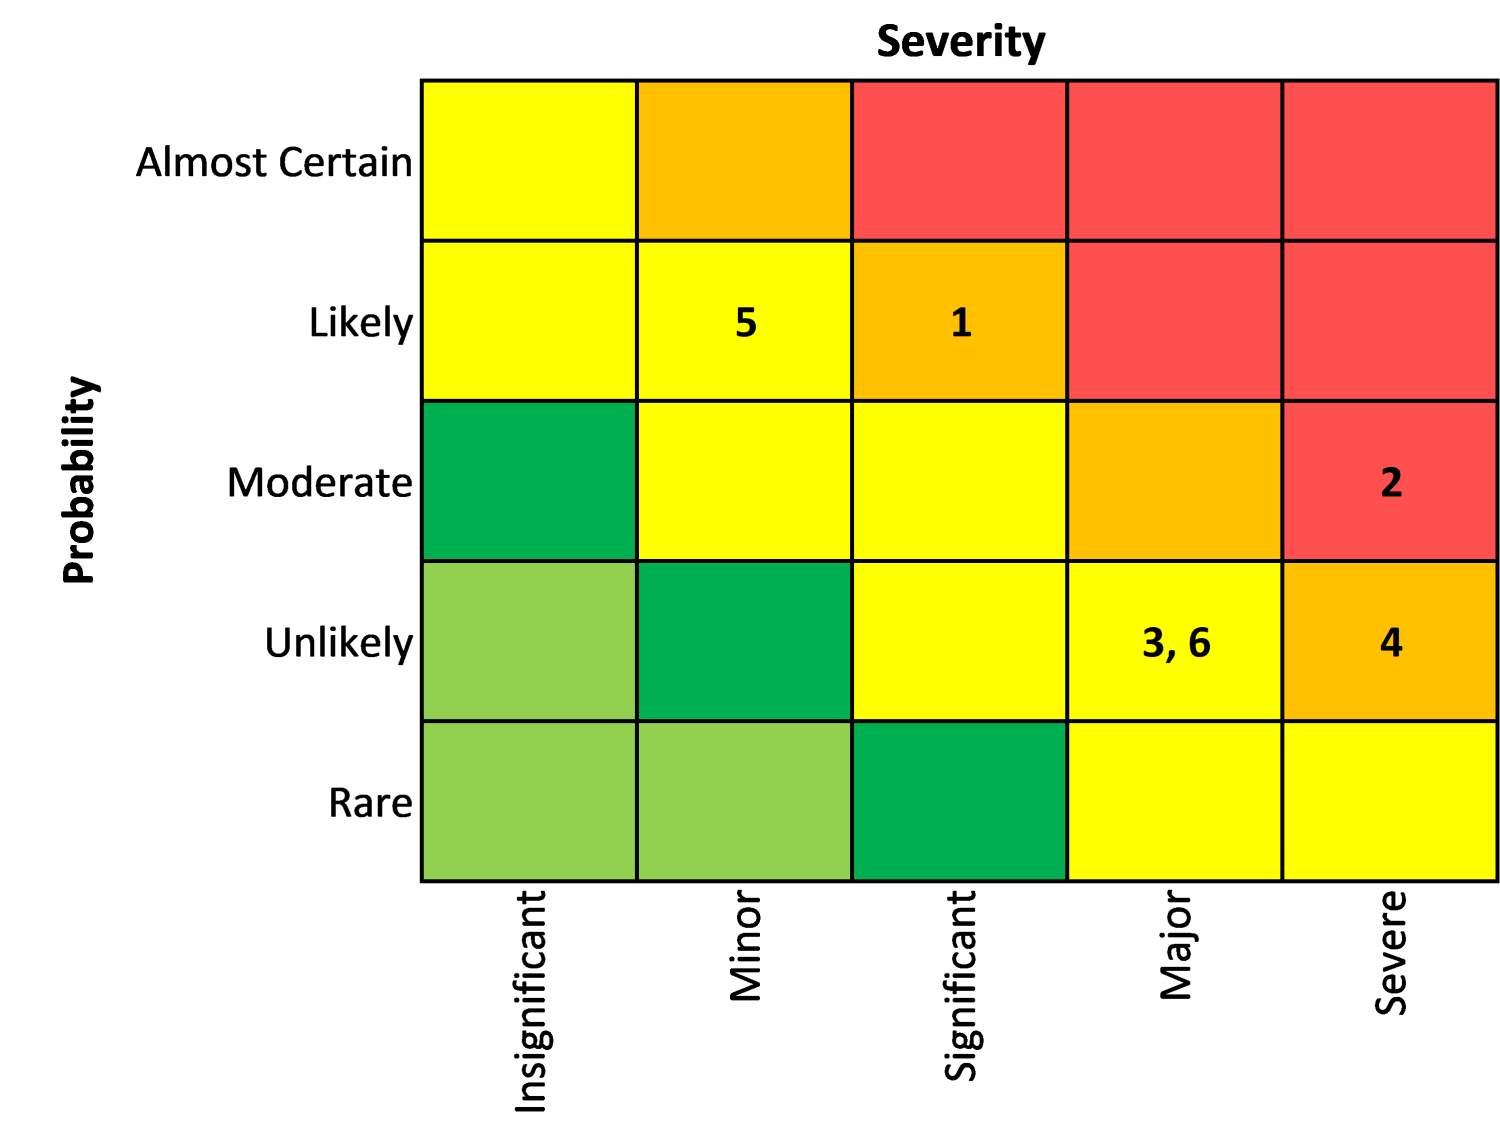
\includegraphics[width=\linewidth]{resources/risks-matrix.png}
  \caption{Risk matrix}
  \label{risk_matrix}
\end{figure}

\begin{table}[]
    \begin{tabular}{llll}
      & Name                                                                           & Severity  & Probability \\
    1 & Finding testing participants                                                   & Medium    & High        \\
    2 & Being able to create reversable programs with additional difficulties          & Very high & Medium      \\
    3 & Not enough time for the actual challenges because of too much programming etc. & High      & Low         \\
    4 & Irreparable corruption of git server.                                          & Very high & Low         \\
    5 & Lost work due to unpushed work.                                                & Low       & High        \\
    6 & License problems with used software.                                           & High      & Low        
    \end{tabular}
\end{table}

Based on these risks we planned steps to mitigate some of the risks.

\begin{table}[]
    \begin{tabular}{lllll}
      & Mitigations                                                               & Actions taken                                    & New severity & New probability \\
    1 & Early looking for participants                                            & Immediately looked for people and found some     & -            & Low             \\
    2 & Having someone with good knowledge available                              & Ivan assured that we can always reach out to him & -            & Low             \\
    3 & Creating the challenges in chronological order and in a iterating fashion &                                                  & -            & Very Low        \\
    4 & Weekly off-site git server backups                                        & Repository mirrored to GitHub                    & Low          & -               \\
    5 & Frequent reminders to push changes                                        &                                                  & -            & Low             \\
    6 & Trying to use opensource or public programs                               &                                                  & -            & Low            
    \end{tabular}
\end{table}
